%% Charlie Redmon
%% 20170914
%% Checkerboard (demonstrating use of foreach loop)

% standalone class for individual image to be included in a document
% border=15pt controls the whitespace padding around the diagram
\documentclass[border=15pt]{standalone}
\usepackage{tikz}

\begin{document}

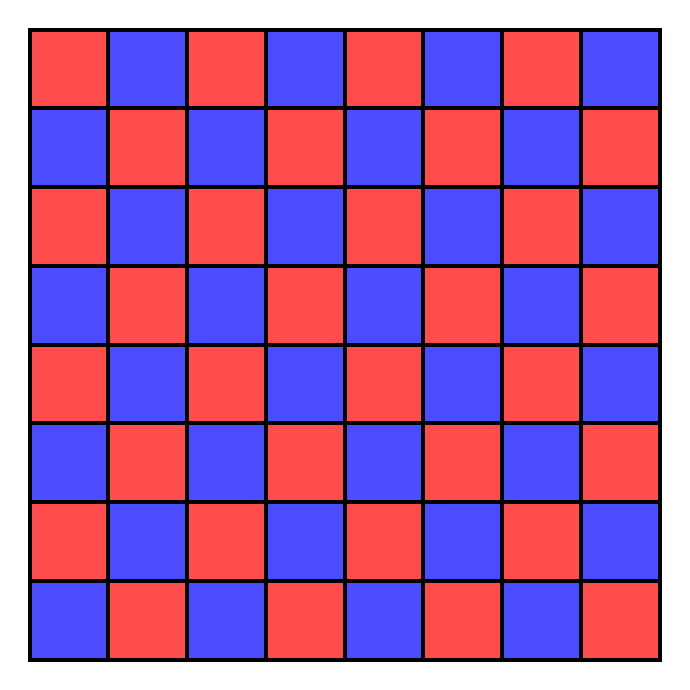
\begin{tikzpicture}
  % large red square for background
  \filldraw[fill=red!70, draw=black, line width=0.5mm] (-4,-4)
  rectangle (4,4);

  % blue squares on the even numbered rows/columns
  \foreach \x in {-4,-2,...,2} {
    \foreach \y in {-4,-2,...,2} {
        \filldraw[fill=blue!70,draw=black,line width=0.5mm] (\x,\y)
        rectangle ++(1,1);
      }
  }

  % blue squares on odd numbered rows/columns
  \foreach \x in {-3,-1,...,3} {
    \foreach \y in {-3,-1,...,3} {
        \filldraw[fill=blue!70,draw=black,line width=0.5mm] (\x,\y)
        rectangle ++(1,1);
    }
  }

\end{tikzpicture}


\end{document}
